% Created 2017-06-14 水 17:45
\documentclass[presentation,dvipdfmx,CJKbookmarks]{beamer}
\usepackage{CJKutf8}
\usepackage[utf8]{inputenc}
\usepackage[T1]{fontenc}
\usepackage{fixltx2e}
\usepackage{graphicx}
\usepackage[export]{adjustbox}
\usepackage{longtable}
\usepackage{float}
\usepackage{wrapfig}
\usepackage{rotating}
\usepackage[normalem]{ulem}
\usepackage{amsmath}
\usepackage{textcomp}
\usepackage{marvosym}
\usepackage{wasysym}
\usepackage{amssymb}
\usepackage{hyperref}
\tolerance=1000
\usepackage{minted}
\usetheme{Berkeley}
\usecolortheme{lily}
\author{\text{\includegraphics[width=1em,valign=t,raise=0.1em]{/home/bhj/src/github/private-config/Wrench-cache/smartisan.png.ps}} 包昊军}
\date{2017-05-08}
\title{\text{\includegraphics[width=1em,valign=t,raise=0.1em]{/home/bhj/src/github/Wrench/release/emojis/iphone-new/PERSONAL_COMPUTER.png.ps}}、\text{\includegraphics[width=1em,valign=t,raise=0.1em]{/home/bhj/src/github/Wrench/release/emojis/iphone-new/MOBILE_PHONE.png.ps}}、\text{\includegraphics[width=1em,valign=t,raise=0.1em]{/home/bhj/src/github/Wrench/release/emojis/iphone-new/WRENCH.png.ps}}}
\hypersetup{
  pdfkeywords={},
  pdfsubject={},
  pdfcreator={Emacs 25.2.1 (Org mode 8.2.10)}}
\AtBeginDvi{\special{pdf:tounicode UTF8-UCS2}}
\begin{document}
\begin{CJK*}{UTF8}{simsun}

\maketitle
\begin{frame}{Outline}
\tableofcontents
\end{frame}

\CJKtilde

\section{什么是小扳手?}
\label{sec-1}

\begin{frame}[label=sec-1-1]{在\text{\includegraphics[width=1em,valign=t,raise=0.1em]{/home/bhj/src/github/Wrench/release/emojis/iphone-new/DESKTOP_COMPUTER.png.ps}}上连接、操作安卓\text{\includegraphics[width=1em,valign=t,raise=0.1em]{/home/bhj/src/github/Wrench/release/emojis/iphone-new/MOBILE_PHONE.png.ps}}}
\begin{block}{\text{\includegraphics[width=1em,valign=t,raise=0.1em]{/home/bhj/src/github/Wrench/release/emojis/iphone-new/WRENCH.png.ps}}能干什么?}
\begin{itemize}
\item 让\text{\includegraphics[width=1em,valign=t,raise=0.1em]{/home/bhj/src/github/Wrench/release/emojis/iphone-new/PERSONAL_COMPUTER.png.ps}}版的QQ一样使用所有\text{\includegraphics[width=1em,valign=t,raise=0.1em]{/home/bhj/src/github/Wrench/release/emojis/iphone-new/MOBILE_PHONE.png.ps}}聊天软件、社交软件
\item 让\text{\includegraphics[width=1em,valign=t,raise=0.1em]{/home/bhj/src/github/Wrench/release/emojis/iphone-new/MOBILE_PHONE.png.ps}}小屏幕变大,屏幕同步到\text{\includegraphics[width=1em,valign=t,raise=0.1em]{/home/bhj/src/github/Wrench/release/emojis/iphone-new/DESKTOP_COMPUTER.png.ps}}上
\item 在\text{\includegraphics[width=1em,valign=t,raise=0.1em]{/home/bhj/src/github/Wrench/release/emojis/iphone-new/DESKTOP_COMPUTER.png.ps}}上显示、处理\text{\includegraphics[width=1em,valign=t,raise=0.1em]{/home/bhj/src/github/Wrench/release/emojis/iphone-new/MOBILE_PHONE.png.ps}}上的通知消息
\item 方便的\thinspace Lua\thinspace 脚本扩展功能
\item 自动抢红包\text{\includegraphics[width=1em,valign=t,raise=0.1em]{/home/bhj/src/github/Wrench/release/emojis/new-emojis/QQ-XIEYANXIAO.PNG}}\text{\includegraphics[width=1em,valign=t,raise=0.1em]{/home/bhj/src/github/Wrench/release/emojis/new-emojis/QQ-MAIMENG.PNG}}
\end{itemize}
\end{block}

\begin{block}{谁会用\text{\includegraphics[width=1em,valign=t,raise=0.1em]{/home/bhj/src/github/Wrench/release/emojis/iphone-new/WRENCH.png.ps}}\text{\includegraphics[width=1em,valign=t,raise=0.1em]{/home/bhj/src/github/Wrench/release/emojis/qq-emojis/smiley_32.png.ps}}}
\begin{itemize}
\item 经常使用\text{\includegraphics[width=1em,valign=t,raise=0.1em]{/home/bhj/src/github/Wrench/release/emojis/iphone-new/PERSONAL_COMPUTER.png.ps}}、用着\text{\includegraphics[width=1em,valign=t,raise=0.1em]{/home/bhj/src/github/Wrench/release/emojis/iphone-new/PERSONAL_COMPUTER.png.ps}}又想着\text{\includegraphics[width=1em,valign=t,raise=0.1em]{/home/bhj/src/github/Wrench/release/emojis/iphone-new/MOBILE_PHONE.png.ps}},用着\text{\includegraphics[width=1em,valign=t,raise=0.1em]{/home/bhj/src/github/Wrench/release/emojis/iphone-new/MOBILE_PHONE.png.ps}}又想着\text{\includegraphics[width=1em,valign=t,raise=0.1em]{/home/bhj/src/github/Wrench/release/emojis/iphone-new/PERSONAL_COMPUTER.png.ps}}
\item \text{\includegraphics[width=1em,valign=t,raise=0.1em]{/home/bhj/src/github/Wrench/release/emojis/iphone-new/NERD_FACE.png.ps}}
\end{itemize}
\end{block}
\end{frame}
\section{屏幕同步}
\label{sec-2}
\begin{frame}[label=sec-2-1]{屏幕同步一:演示模式}
\includegraphics[width=.9\linewidth]{./images/wrench-demo.ps}
\begin{itemize}
\item 各个\text{\includegraphics[width=1em,valign=t,raise=0.1em]{/home/bhj/src/github/Wrench/release/emojis/iphone-new/RADIO_BUTTON.png.ps}}功能\text{\includegraphics[width=1em,valign=t,raise=0.1em]{/home/bhj/src/github/Wrench/release/emojis/iphone-new/ELECTRIC_LIGHT_BULB.png.ps}}
\end{itemize}
\end{frame}

\begin{frame}[label=sec-2-2]{屏幕同步二:高清阅读模式}
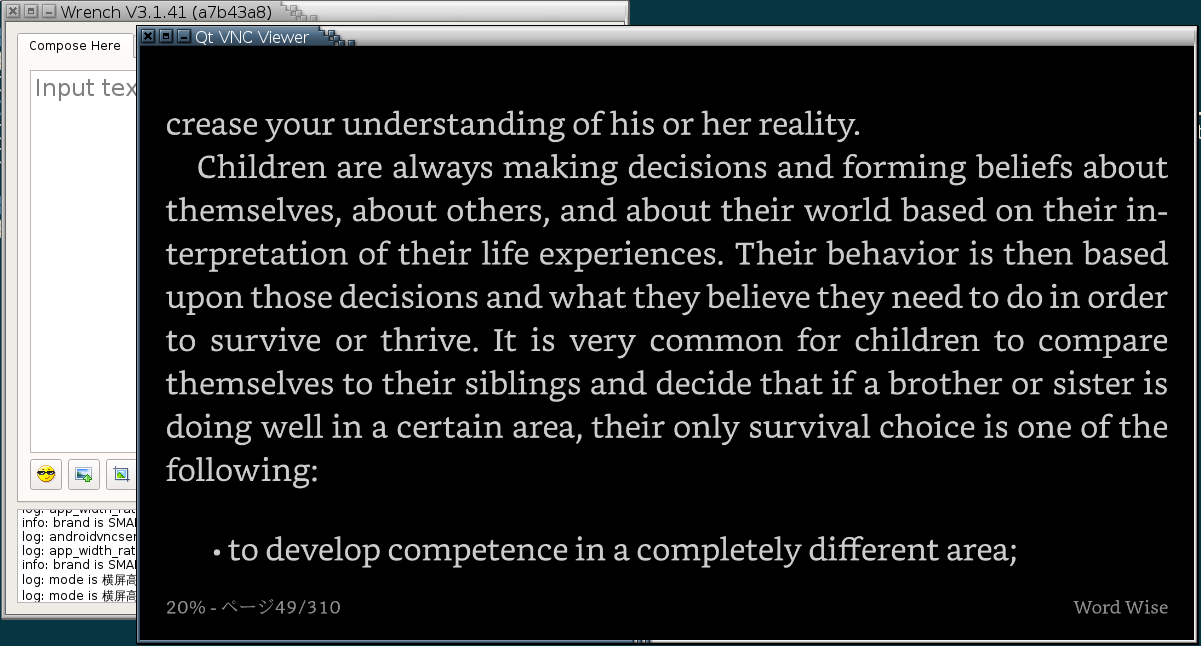
\includegraphics[width=.9\linewidth]{./images/wrench-read.ps}
\end{frame}

\begin{frame}[label=sec-2-3]{Why\text{\includegraphics[width=1em,valign=t,raise=0.1em]{/home/bhj/src/github/Wrench/release/emojis/qq-emojis/smiley_32.png.ps}}}
\begin{block}{手机上看书太\text{\includegraphics[width=1em,valign=t,raise=0.1em]{/home/bhj/src/github/Wrench/release/emojis/iphone-new/TIRED_FACE.png.ps}}了!}
\end{block}
\begin{block}{手机上看书太容易\text{\includegraphics[width=1em,valign=t,raise=0.1em]{/home/bhj/src/github/Wrench/release/emojis/iphone-new/BROKEN_HEART.png.ps}}了!}
\begin{itemize}
\item 一不小心就把\text{\includegraphics[width=1em,valign=t,raise=0.1em]{/home/bhj/src/github/private-config/Wrench-cache/com.sina.weibo.SplashActivity.png.ps}}打开
\item 一不小心就把\text{\includegraphics[width=1em,valign=t,raise=0.1em]{/home/bhj/src/github/private-config/Wrench-cache/com.tencent.mm.ui.LauncherUI.png.ps}}朋友圈打开
\end{itemize}
\end{block}
\begin{block}{不是有网页版\thinspace Kindle Reader\thinspace 吗?}
\begin{itemize}
\item 跟手持\thinspace Kindle\thinspace 设备间的同步非常折磨神经\text{\includegraphics[width=1em,valign=t,raise=0.1em]{/home/bhj/src/github/Wrench/release/emojis/qq-emojis/smiley_19.png.ps}}
\end{itemize}
\end{block}
\begin{block}{跟\thinspace \href{https://github.com/baohaojun/system-config}{system-config}\thinspace 结合,手机上的金山词霸?}
\end{block}
\end{frame}

\section{自动操作手机}
\label{sec-3}
\begin{frame}[label=sec-3-1]{聊天}
\begin{block}{发送文字\text{\includegraphics[width=1em,valign=t,raise=0.1em]{/home/bhj/src/github/Wrench/release/emojis/iphone-new/FACE_WITH_ROLLING_EYES.png.ps}}}
\begin{itemize}
\item 在手机上自动查找\text{\includegraphics[width=1em,valign=t,raise=0.1em]{/home/bhj/src/github/private-config/Wrench-cache/com.tencent.mobileqq.activity.SplashActivity.png.ps}}、\text{\includegraphics[width=1em,valign=t,raise=0.1em]{/home/bhj/src/github/private-config/Wrench-cache/com.tencent.mm.ui.LauncherUI.png.ps}}联系人并打开聊天界面
\end{itemize}
\end{block}
\begin{block}{发送表情符\text{\includegraphics[width=1em,valign=t,raise=0.1em]{/home/bhj/src/github/Wrench/release/emojis/new-emojis/QQ-DOGE.PNG}}}
\end{block}
\begin{block}{发送图片\text{\includegraphics[width=1em,valign=t,raise=0.1em]{/home/bhj/src/github/Wrench/release/emojis/iphone-new/FRAME_WITH_PICTURE.png.ps}}}
\begin{itemize}
\item 选图片文件
\item 从浏览器直接拖图(像不像\text{\includegraphics[width=1em,valign=t,raise=0.1em]{/home/bhj/src/github/private-config/Wrench-cache/com.smartisanos.sidebar.setting.SettingActivity.png.ps}}\text{\includegraphics[width=1em,valign=t,raise=0.1em]{/home/bhj/src/github/Wrench/release/emojis/qq-emojis/smiley_32.png.ps}})
\item 从\text{\includegraphics[width=1em,valign=t,raise=0.1em]{/home/bhj/src/github/private-config/Wrench-cache/com.sina.weibo.SplashActivity.png.ps}}网页上怎么看问答\text{\includegraphics[width=1em,valign=t,raise=0.1em]{/home/bhj/src/github/Wrench/release/emojis/qq-emojis/smiley_32.png.ps}}
\end{itemize}
\end{block}
\end{frame}

\begin{frame}[label=sec-3-2]{搜索}
\begin{block}{找\text{\includegraphics[width=1em,valign=t,raise=0.1em]{/home/bhj/src/github/private-config/Wrench-cache/com.tencent.mm.ui.LauncherUI.png.ps}}联系人}
\end{block}
\begin{block}{找\text{\includegraphics[width=1em,valign=t,raise=0.1em]{/home/bhj/src/github/private-config/Wrench-cache/com.tencent.mobileqq.activity.SplashActivity.png.ps}}联系人}
\end{block}
\begin{block}{找\text{\includegraphics[width=1em,valign=t,raise=0.1em]{/home/bhj/src/github/private-config/Wrench-cache/com.tencent.mobileqq.activity.SplashActivity.png.ps}}群里的联系人}
\end{block}
\begin{block}{找\text{\includegraphics[width=1em,valign=t,raise=0.1em]{/home/bhj/src/github/private-config/Wrench-cache/com.sina.weibo.SplashActivity.png.ps}}上的用户}
\end{block}
\begin{block}{按发件人找\text{\includegraphics[width=1em,valign=t,raise=0.1em]{/home/bhj/src/github/private-config/Wrench-cache/com.android.email.activity.Welcome.png.ps}}}
\end{block}
\begin{block}{在\text{\includegraphics[width=1em,valign=t,raise=0.1em]{/home/bhj/src/github/private-config/Wrench-cache/com.amazon.kindle.UpgradePage.png.ps}}里搜书}
\end{block}
\end{frame}

\begin{frame}[label=sec-3-3]{扫码}
\begin{block}{\text{\includegraphics[width=1em,valign=t,raise=0.1em]{/home/bhj/src/github/private-config/Wrench-cache/com.tencent.mm.ui.LauncherUI.png.ps}}扫码}
\end{block}
\begin{block}{\text{\includegraphics[width=1em,valign=t,raise=0.1em]{/home/bhj/src/github/private-config/Wrench-cache/com.sina.weibo.SplashActivity.png.ps}}扫码}
\end{block}
\begin{block}{\text{\includegraphics[width=1em,valign=t,raise=0.1em]{/home/bhj/src/github/private-config/Wrench-cache/com.jingdong.app.mall.main.MainActivity.png.ps}}扫码}
\end{block}
\end{frame}

\begin{frame}[label=sec-3-4]{抢红包}
\begin{block}{抢\text{\includegraphics[width=1em,valign=t,raise=0.1em]{/home/bhj/src/github/private-config/Wrench-cache/com.tencent.mm.ui.LauncherUI.png.ps}}红包(并自动表示\text{\includegraphics[width=1em,valign=t,raise=0.1em]{/home/bhj/src/github/Wrench/release/emojis/iphone-new/PERSON_BOWING_DEEPLY.0.png.ps}})}
\end{block}
\begin{block}{抢\text{\includegraphics[width=1em,valign=t,raise=0.1em]{/home/bhj/src/github/private-config/Wrench-cache/com.tencent.mobileqq.activity.SplashActivity.png.ps}}红包}
\end{block}
\end{frame}

\section{高级用法}
\label{sec-4}
\begin{frame}[label=sec-4-1]{自己录\thinspace Lua\thinspace 脚本}
\begin{block}{用鼠标右键点击屏幕同步窗口}
\includegraphics[width=.9\linewidth]{./images/wrench-screen-record.ps}
\end{block}
\end{frame}

\begin{frame}[label=sec-4-2]{注意事项}
\begin{block}{屏幕同步高清阅读模式目前只支持坚果\thinspace Pro}
\end{block}
\begin{block}{确保安卓\thinspace adb\thinspace 连接}
\end{block}
\begin{block}{通知消息同步可能要打开关闭多试几次}
\end{block}
\begin{block}{下载地址}
\href{https://github.com/SmartisanTech/Wrench-releases/releases}{Github SmartisanTech Wrench-Releases}
\end{block}
\end{frame}
\section{开源信息}
\label{sec-5}
\begin{frame}[label=sec-5-1]{Wrench\thinspace 是开源项目}
\begin{block}{项目\thinspace github\thinspace 网址}
\url{https://github.com/SmartisanTech/Wrench}
\end{block}

\begin{block}{使用\thinspace Qt、Lua\thinspace 编程,支持所有主流\thinspace PC\thinspace 平台}
\begin{itemize}
\item Linux
\item Mac
\item Windows
\end{itemize}
\end{block}

\begin{block}{支持几乎所有安卓手机}
\begin{itemize}
\item 支持\text{\includegraphics[width=1em,valign=t,raise=0.1em]{/home/bhj/src/github/private-config/Wrench-cache/smartisan.png.ps}}所有机型
\item 其他厂商手机最低安卓版本要求请参考\thinspace Smartisan T1
\end{itemize}
\end{block}
\end{frame}

\begin{frame}[label=sec-5-2]{致谢、Howto Contribute}
\begin{block}{致谢}
\begin{itemize}
\item \text{\includegraphics[width=1em,valign=t,raise=0.1em]{/home/bhj/src/github/private-config/Wrench-cache/smartisan.png.ps}} \href{http://www.smartisan.com/cn/}{锤子科技}
\end{itemize}
\end{block}
\begin{block}{Help Wrench Project}
\begin{itemize}
\item 源代码\thinspace Patch、\text{\includegraphics[width=1em,valign=t,raise=0.1em]{/home/bhj/src/github/Wrench/release/emojis/qq-emojis/smiley_73.png.ps}}修正
\item Ideas are welcome\text{\includegraphics[width=1em,valign=t,raise=0.1em]{/home/bhj/src/github/Wrench/release/emojis/iphone-new/HEAVY_HEART_EXCLAMATION_MARK_ORNAMENT.png.ps}}
\item 购买、使用锤子科技手机(当前版本用坚果\thinspace Pro\thinspace 开发)
\item 求转发\text{\includegraphics[width=1em,valign=t,raise=0.1em]{/home/bhj/src/github/Wrench/release/emojis/weibo-emojis/lxh_qiuguanzhu.png.ps}}、帮助更多朋友使用小扳手
\item 用小扳手给作者打钱\text{\includegraphics[width=1em,valign=t,raise=0.1em]{/home/bhj/src/github/Wrench/release/emojis/qq-emojis/smiley_32.png.ps}}\text{\includegraphics[width=1em,valign=t,raise=0.1em]{/home/bhj/src/github/Wrench/release/emojis/new-emojis/wx-WuLian.PNG}}
\item 微信公众号: Programate
\end{itemize}

\end{block}
\end{frame}
% Emacs 25.2.1 (Org mode 8.2.10)
\end{CJK*}
\end{document}
